\documentclass{report}
\usepackage[utf8]{inputenc}    
\usepackage[T1]{fontenc}
\usepackage[francais]{babel}
\usepackage{wrapfig}
\usepackage{graphicx}
\usepackage{listings,xcolor}
\usepackage{appendix}
\usepackage{adjustbox}
\usepackage{titling}
\usepackage{float}
\usepackage{pdfpages}
\usepackage{caption}
\usepackage{subcaption}
\usepackage[hidelinks]{hyperref}

\hypersetup{
    colorlinks,
    citecolor=black,
    filecolor=black,
    linkcolor=blue,
    urlcolor=blue
}

%Géométrie des pages
\usepackage{geometry}
\geometry{hmargin=1.9cm,vmargin=1.9cm}

%Définition des couleurs pour le code xml
\definecolor{colorxmlnode}{rgb}{0.2, 0.2, 0.2} 
\definecolor{maroon}{RGB}{178 34 34}


%Profondeur des compteurs et de la tableofcontents
\setcounter{secnumdepth}{3}
\setcounter{tocdepth}{2}


%lst xml
\lstdefinelanguage{XML}
{
  basicstyle=\ttfamily,
  morestring=[s]{"}{"},
  morecomment=[s]{?}{?},
  morecomment=[s]{!--}{--},
  commentstyle=\color{darkgreen},
  moredelim=[s][\color{black}]{>}{<},
  moredelim=[s][\color{red}]{\ }{=},
  stringstyle=\color{blue},
  identifierstyle=\color{maroon}
}


\addto\captionsfrench{%
  \renewcommand\appendixname{Annexe}
  \renewcommand\appendixpagename{Annexes}
}

%Définition des commandes \noeud et \classe
\newcommand\classe[1]{\mbox{\textit{#1}}}
\newcommand\noeud[1]{\textcolor{colorxmlnode}{<\mbox{#1}>}}




\begin{document}

\begin{titlepage}
	\centering
	
    \vspace*{1.2 cm}
    
   	\textsc{\LARGE Master i informatique\\Design Pattern\\[0.3cm]\large Décembre 2017}

	\vspace{2.2cm}
    
    
    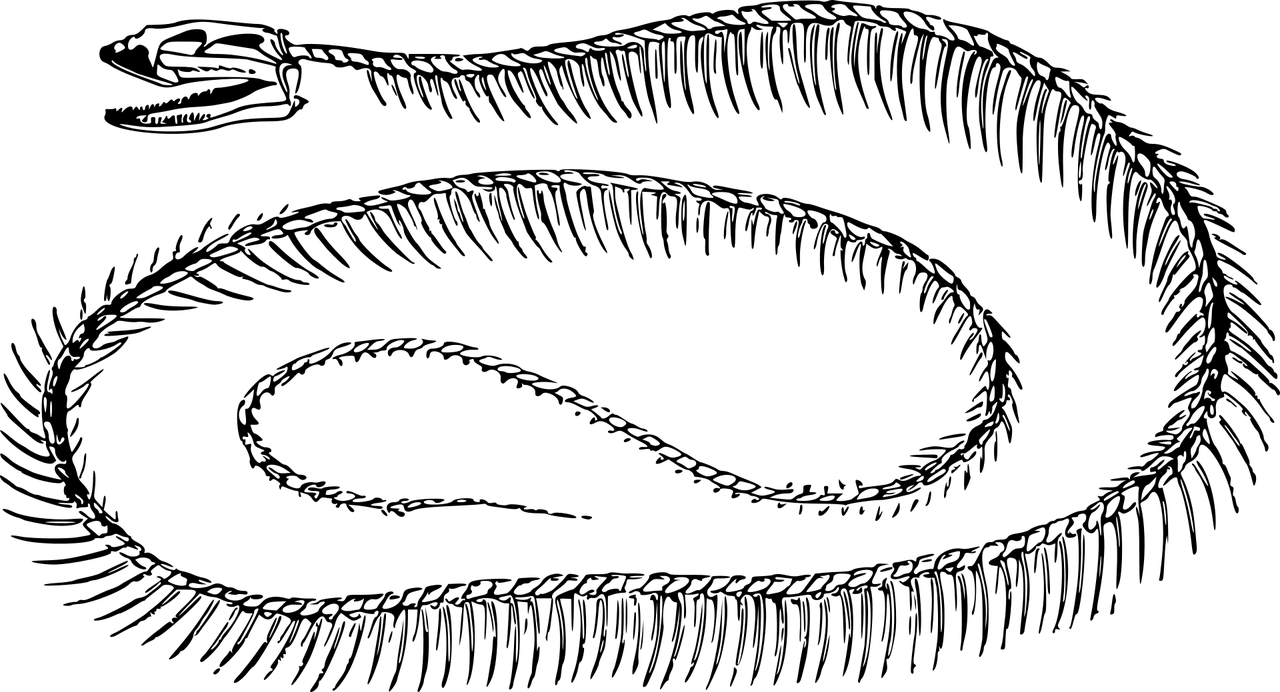
\includegraphics[scale = 0.29]{img/snake.png}\\[0.5 cm]
	\rule{\linewidth }{0.2 mm} \\[0.15 cm]
    {\LARGE \textbf{Projet de Développement}\\[0.2cm] \large
		\textbf{Snake en réseau}}\\
	\rule{\linewidth}{0.2 mm}
       \vspace*{0.1 cm}
	
	\begin{center}
	\vspace{0.3cm}
	
	\emph{Auteurs}\\
	\vspace{0.1cm}
	David \bsc{Dembele}\\ 
	Alassane \bsc{Diop}\\
	Rahmatou Walet \bsc{Mohamedoun}
		
	\vspace{0.5cm}
	\emph{Professeur}\\
	\vspace{0.1cm}
	Benoit \bsc{Da Mota}
	\end{center}		
	
		
	\vspace{1.5cm}
	\hspace{15cm}
\includegraphics[scale = 0.1]{img/logo.png}

    
    
\end{titlepage}


\tableofcontents

\chapter{Introduction}

	\section{Contexte}
		\par
Dans le cadre de l'UE Design Pattern, de notre premier semestre de Master 1 Informatique à l'Université d'Angers, nous avons poursuivi la phase d'analyse d'un développement de jeu de Snake en réseau. \label{contexte}
	
	\section{Objectifs}
		\par
L'objectif attendu est de permettre à différents joueurs de se connecter au jeu et de jouer entre eux.
Chaque joueur doit disposer d'un serpent qu'il contrôle à l'aide du clavier, avec les touches de direction (HAUT, BAS, GAUCHE, DROITE). Le serpent doit se déplacer pour ramasser des bonus; ces bonus lui permettent de grandir, éventuellement de devenir momentanément invisible, d'augmenter ses points de vie, de faire un retour dans le temps pendant un certains nombre de secondes.\\
Les serpents pourront s'entre-tuer; un serpent tué se transforme en bonus en faveur du serpent tueur ainsi le dernier serpent à survivre sera le gagnant.

\par
Le jeu doit permettre aux joueurs de faire des demandes de connexion et de déconnexion, d'envoyer leurs déplacements au serveur.\\
Le serveur doit gérer les connexions et déconnexions des joueurs et centraliser les actions des joueurs. En effet il gère le plan de jeu partagé par tous les joueurs.\\
À chaque connexion d'un joueur, le serveur doit récupérer les informations du joueur, lui attribuer un serpent, son niveau de compétence et son niveau de jeu.\\
À chaque déplacement d'un serpent, il doit faire une mise à jour du plan de jeu pour prendre en compte la nouvelle position du serpent, en informer les autres joueurs. \label{objectifs}

\chapter{Protocole réseau}
	
	\section{Motivation}
		\par
Dans ce jeu, nous avons utilisé les protocoles TCP\footnote{Transmission Control Protocol (littéralement, « protocole de contrôle de transmissions »), abrégé TCP, est un protocole de transport fiable, en mode connecté. Wikipédia} et UDP\footnote{Le User Datagram Protocol (UDP, en français protocole de datagramme utilisateur) est un des principaux protocoles de télécommunication utilisés par Internet. Il fait partie de la couche transport du modèle OSI, il appartient à la couche 4, comme TCP. Wikipédia}.

\par
Le protocole UDP nous sert dans le cas d'une transmission sans accusé de réception; en effet le protocole UDP repose sur une communication unidirectionnelle. Lorsqu'une machine A envoie un paquet à une machine B, les paquets sont reçus par B sans accusé de réception vers la machine A.

\par
Contrairement au protocole UDP, le protocole TCP repose sur une communication bidirectionnelle. La communication entre deux machines nécessite toujours un accusé de réception du récepteur vers l'émetteur. Dans le cas d'une communication où il faudra limiter la perte de paquet, TCP pourra nous servir. \\ \label{motivation}

	\section{Justification}
		\par
Le protocole UDP est utilisé dans les cas suivants :
\begin{itemize}
	\item déconnexion : lorsqu'un joueur souhaite quitter le jeu il envoie une requête de déconnexion au serveur, le serveur reçoit la requête et lui déconnecte du jeu sans lui en informer (sans accusé de réception).
	
	\item envoi du plan de jeu : lorsque le serveur centralise les actions des utilisateurs, il met à jour le plan du jeu et l'envoie aux joueurs; cette opération peut être répétée autant de fois possible sans perturber le jeu.\\
\end{itemize}
Les informations destinées aux joueurs en provenance du serveur, seront envoyées via le broadcast\footnote{Le broadcast permet au serveur d'envoyer un paquet à tous le joueurs connectés}. \\

\par
Le protocole TCP est utilisé à chaque fois qu'il y ait échange entre le serveur et les joueurs sauf dans le cas d'une déconnexion ou d'un envoi du plan de jeu.\\

Les échanges d'informations entre le serveur et les joueurs se feront via des sockets et doivent être fiables, sans erreurs notamment dans le cas d'une connexion d'un joueur au serveur, de la réception par le serveur des actions des joueurs. 
La communication entre le serveur et les joueurs reposent sur des requêtes HTTP. Ci dessous une représentation de cette communication : 

\begin{figure}[ht]
	\centering
	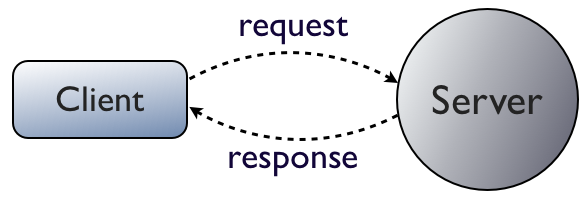
\includegraphics[scale = 0.29]{img/communicationHTTP.png}
	\caption{Communication entre joueur (client) et le serveur}
\end{figure} \label{justification}

	\section{Éventuels problèmes}
		\par
Assurer les communications entre les joueurs et le serveur, en essayant de garantir l'intégrité des paquets, s'avère complexe; des erreurs liées à la transmission des paquets peuvent survenir.\\
En effet, à la fin d'une partie, il peut y avoir un paquet renseignant la position ou le déplacement d'un serpent; si ce paquet arrive après la réception du paquet indiquant la fin de la partie, le joueur émettant le paquet pourrait être bloqué. \\ \label{problemes}
	
	\section{Implémentation}
		\input{Protocole/implementation.tex} \label{implementation}
		

\chapter{Conception}
			
	\section{Cas d'utilisation}
			\par
Les échanges entre les joueurs et le serveur peuvent être résumés par les cas d'utilisation suivants où les acteurs sont les joueurs : 

\begin{itemize}

	\item Se Connecter
	\item Entrer son nom
	\item Deconnecter
	\item Creer une partie de jeu
	\item Initialiser le jeu
	\item Jouer
	\item Consulter l'aide
	\item Consulter score
	\item Inviter joueur
	\item Quitter le jeu

\end{itemize}

Ci dessous le diagramme des cas d'utilisation : \\

\begin{figure}[ht]
	\centering
	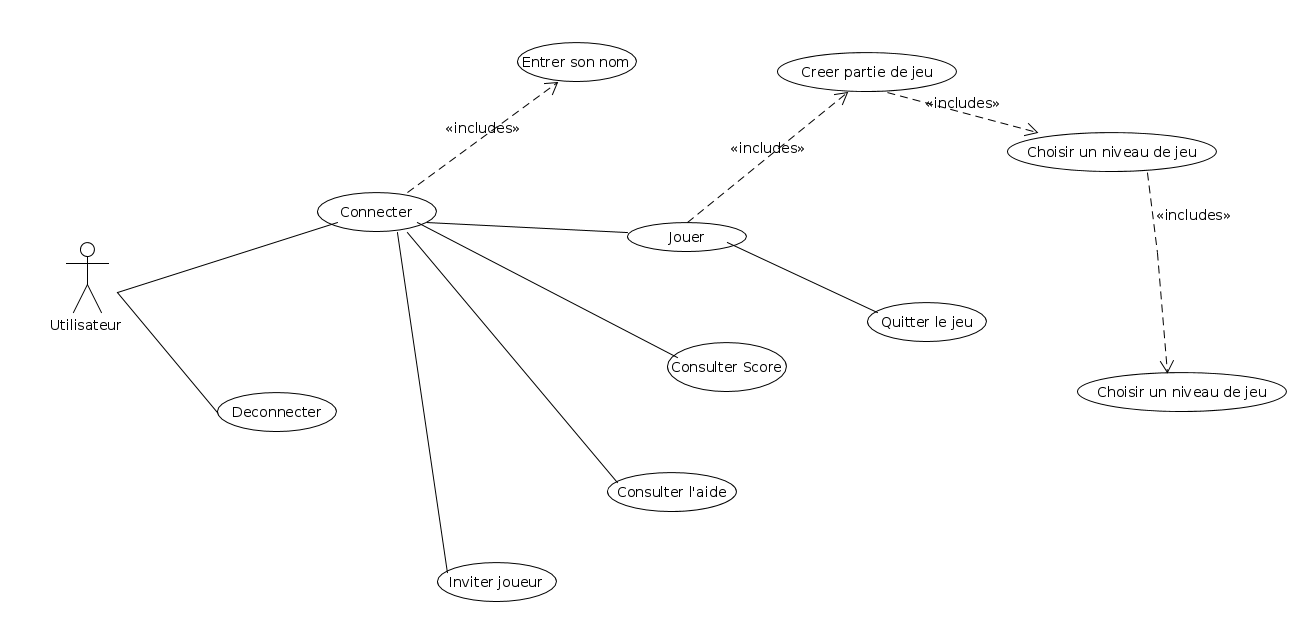
\includegraphics[scale = 0.40]{img/useCase.png}
	\caption{Diagramme des cas d'utilisation}
\end{figure}
 \label{cas_utilisation}
			
	\section{Points de changement et d'évolution}
			\par
Durant une partie de jeu, beaucoup d'objets sont amenés à être modifiés. En effet, les actions effectuées par les joueurs entraînent d'états. Ainsi pour un joueur donné, nous pouvons dire que les points de changement concerne : 

\begin{itemize}

	\item le serpent : le comportement du serpent change; il se déplace, ramasse des bonus, s'allonge au fur et à mesure du jeu. Sa visibilité peut changer ainsi que son nombre de vie.
	
	\item le niveau de jeu : à chaque fin de partie, les joueurs peuvent changer de niveau; ils passent d'un niveau inférieur à un niveau supérieur.
	
	\item le plan de jeu : il change en fonction du niveau de jeu. Chaque niveau de jeu propose un plan de jeu différent, plus complexe.
	
	\item le nombre de joueurs : au début du jeu, il y a un nombre de joueurs défini; ce nombre est amené à évoluer positivement si un joueur rejoint la partie et négativement si le serpent d'un joueur meurt.
	
	\item le score : plus un joueur ramasse des bonus, plus son score augmente.
	
	\item l'accès au serveur : l'accès au serveur d'un joueur peut passer d'un état connecté à un état déconnecté et inversement.
	
	\item une partie de jeu : elle peut passer d'un état début à un état en cours, d'un état en cours à un état pause, d'un état en cours à un état terminé.
	
\end{itemize}
 \label{changement}
			\input{Conception/evolution.tex} \label{evolution}
			
	\section{Design envisagé}
			\par
Notre application repose sur une architecture 3-Tiers\footnote{L'architecture trois tiers, aussi appelée architecture à trois niveaux ou architecture à trois couches, est l'application du modèle plus général qu'est le multi-tier. L'architecture logique du système est divisée en trois niveaux ou couches : couche de présentations, couche de traitement, couche d'accès aux données. C'est une architecture basée sur l'environnement client-serveur. Wikipédia.}\\

Cette architecture nous permet de mieux distinguer chaque partie, d'où une conception plus optimale. Ainsi, nous aurons trois parties distinctes : 

\begin{itemize}

	\item couche client (les joueurs) : cette partie regroupe les joueurs qui se connectent au serveur. Nous aurons une abstraction des joueurs physiques, une représentation des joueurs en mémoire du côté de la couche client. Ci dessous le diagramme de classe de la couche client :

\begin{figure}[!h]
	\centering
	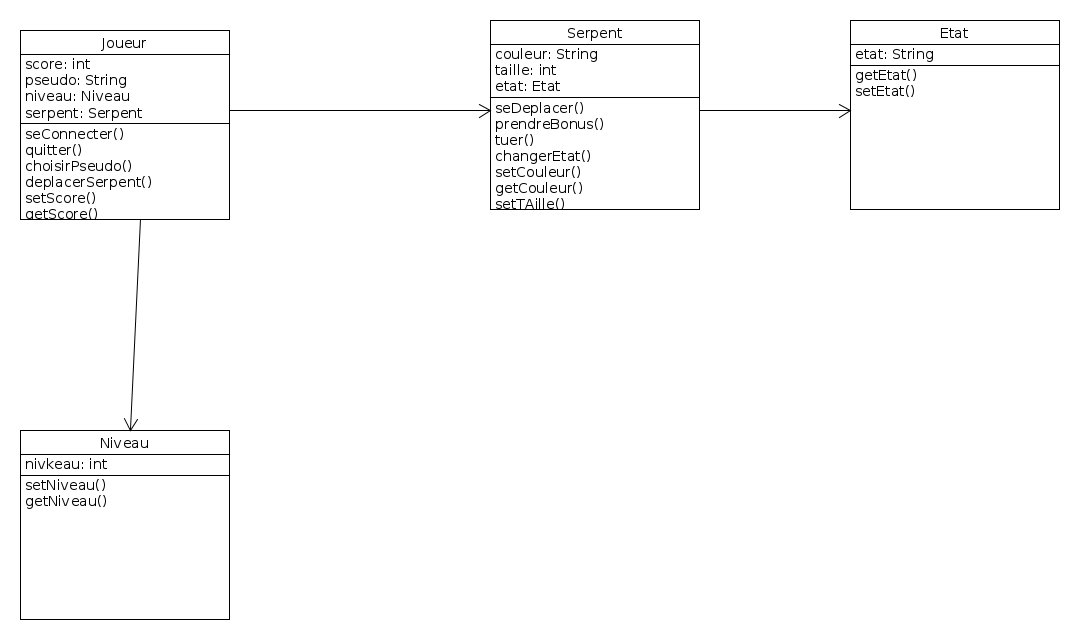
\includegraphics[scale = 0.40]{img/diagClient.png}
	\caption{Diagramme de classe de la couche client}
\end{figure}

	
	\item couche serveur : cette partie regroupe à la fois le serveur, la vue, le modèle (les classes métiers). \\
	Le serveur assure tout ce qui est communication avec les joueurs, centralise leurs actions. Le modèle est une abstraction des joueurs physiques, une représentation des joueurs en mémoire du côté dans la couche serveur. La vue représente le plan, la partie visible qui sera partagée par tous les joueurs, la partie qui permet aux joueurs d'interagir avec le jeu, serveur. \\
	
	Afin de mieux séparer les composants de cette couche, nous structurons cette couche en utilisant le patter MVC, ainsi nous aurons de manière distincte le serveur qui est en même temps le contrôleur, la vue et le modèle. Ci dessous une représentation du pattern MVC :

\begin{figure}[!h]
	\centering
	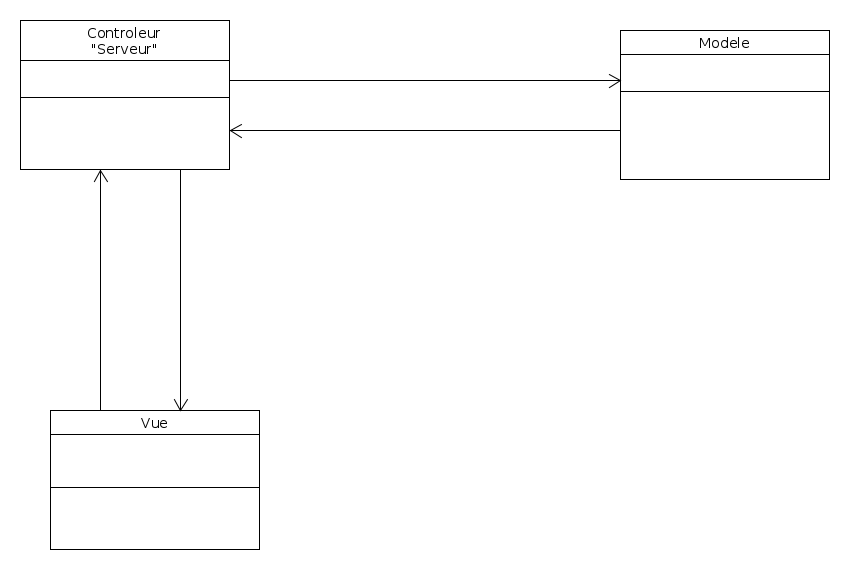
\includegraphics[scale = 0.40]{img/diagMVC.png}
	\caption{Représentation du design pattern MVC}
\end{figure}

	
	Le serveur communique avec la vue et le modèle via le pattern Façade. Ci dessus, le diagramme des classe du pattern MVC intégrant le pattern Façade du serveur :

\begin{figure}[!h]
	\centering
	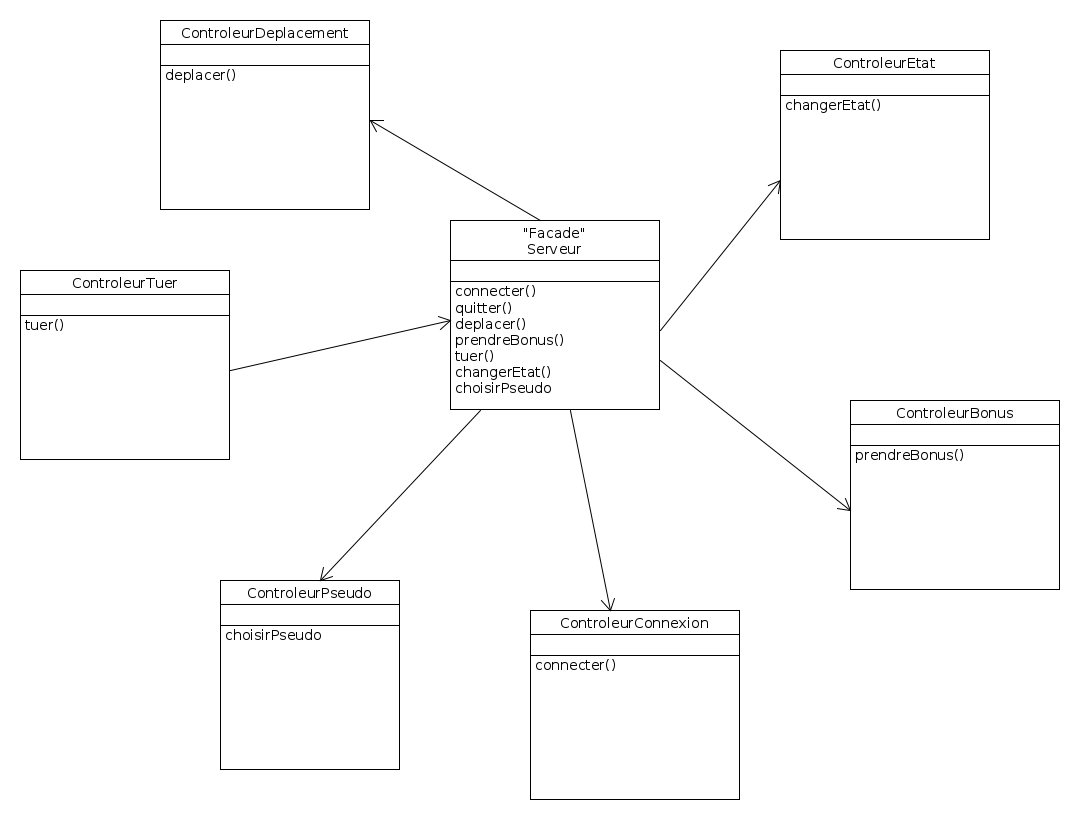
\includegraphics[scale = 0.40]{img/diagServeur.png}
	\caption{Diagramme de classe de la couche serveur}
\end{figure}
\newpage
	
	\item couche persistance : la persistance des données est gérée dans cette partie. \\
	Les données sont une abstraction des joueurs en base de données. Dans cette couche, les données sont des objets des classes métiers. \\
	
\end{itemize}

\par
Pour faire communiquer ces trois couches, nous mettons en place une conception basée sur différents designs patterns. \\

\par
La communication entre la couche client et celle serveur se fera via le pattern Proxy. Ci dessus une représentation de la communication les couches client et serveur :
\begin{figure}[!h]
	\centering
	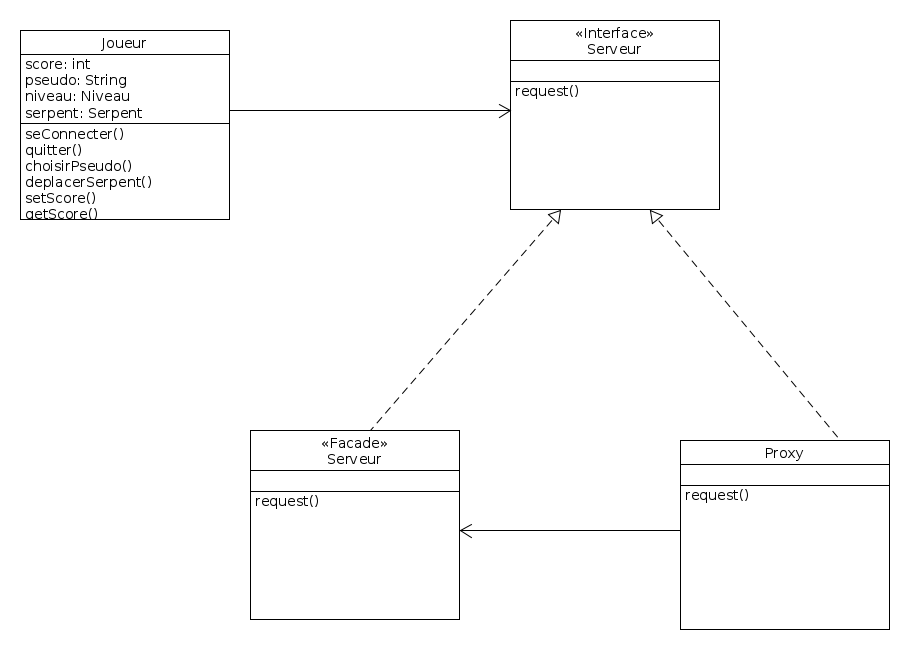
\includegraphics[scale = 0.40]{img/diagProxy.png}
	\caption{Diagramme de classe du pattern Proxy}
\end{figure}
\newpage

\par
La persistance des données passe par le pattern DAO. Ci dessous une représentation de la persistance des données :
\begin{figure}[!h]
	\centering
	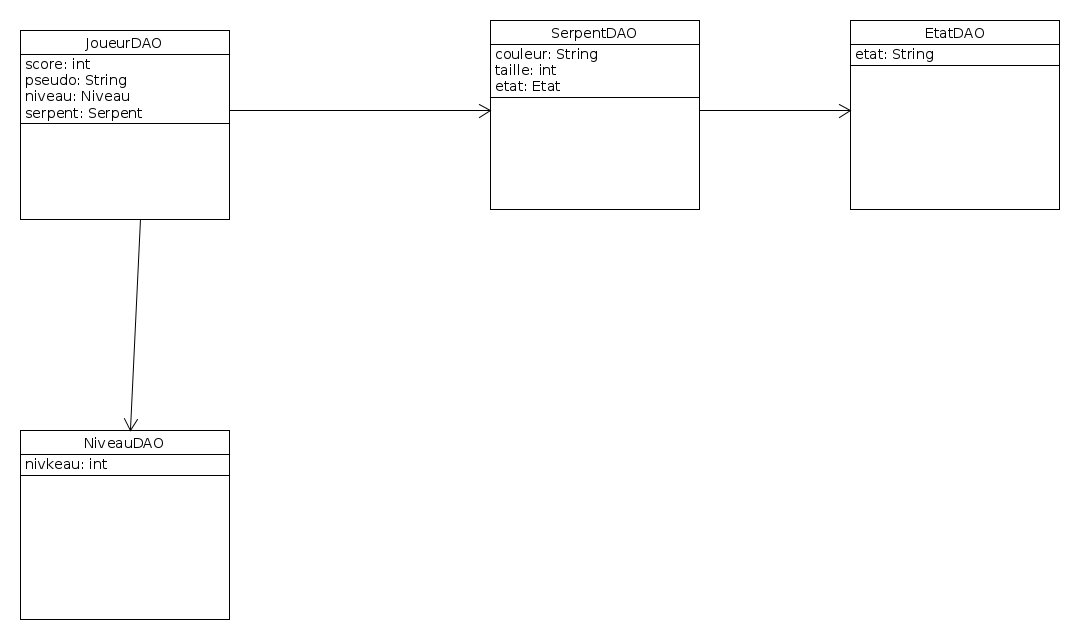
\includegraphics[scale = 0.40]{img/diagDAO.png}
	\caption{Diagramme de classe du pattern DAO}
\end{figure}


 \label{design}
			
	\section{Justification}
			\par
Le protocole UDP est utilisé dans les cas suivants :
\begin{itemize}
	\item déconnexion : lorsqu'un joueur souhaite quitter le jeu il envoie une requête de déconnexion au serveur, le serveur reçoit la requête et lui déconnecte du jeu sans lui en informer (sans accusé de réception).
	
	\item envoi du plan de jeu : lorsque le serveur centralise les actions des utilisateurs, il met à jour le plan du jeu et l'envoie aux joueurs; cette opération peut être répétée autant de fois possible sans perturber le jeu.\\
\end{itemize}
Les informations destinées aux joueurs en provenance du serveur, seront envoyées via le broadcast\footnote{Le broadcast permet au serveur d'envoyer un paquet à tous le joueurs connectés}. \\

\par
Le protocole TCP est utilisé à chaque fois qu'il y ait échange entre le serveur et les joueurs sauf dans le cas d'une déconnexion ou d'un envoi du plan de jeu.\\

Les échanges d'informations entre le serveur et les joueurs se feront via des sockets et doivent être fiables, sans erreurs notamment dans le cas d'une connexion d'un joueur au serveur, de la réception par le serveur des actions des joueurs. 
La communication entre le serveur et les joueurs reposent sur des requêtes HTTP. Ci dessous une représentation de cette communication : 

\begin{figure}[ht]
	\centering
	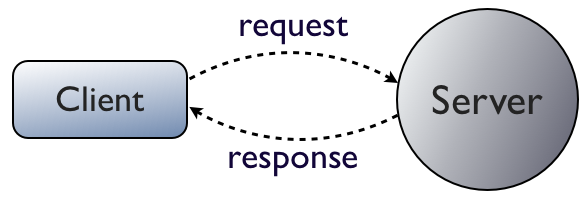
\includegraphics[scale = 0.29]{img/communicationHTTP.png}
	\caption{Communication entre joueur (client) et le serveur}
\end{figure} \label{justification}
			

\chapter{Conclusion}
			
%	\section{Types de QR Codes}
%		\input{Modelisation/typesQRCodes.tex} \label{typesQR}
%		
%	\newpage
%		
%	\section{Représentation des données}
%		\input{Modelisation/representationDonnees.tex} \label{representationDonnees}
%		
%	\section{Stockage des données}
%		\input{Modelisation/stockage.tex} \label{stockage}
%		
%

\end{document}
